\documentclass{article}
\usepackage{amsmath,graphicx,amssymb,amsthm,url}

\title{Implementation Assignment 1}
\date{\today}
\author{Rong Yu and Finn Womack}

\begin{document}
	\maketitle
	\section{Appended 1s column}
	\subsection{Computing W}
After loading the data into X matrices and Y vectors we appended a column of ones to Xs and calculated W in the following way:
	$$
	W = (X_{train}^{T}X_{train})^{-1}X_{train}^{T}Y_{train}
	$$
	The resulting vector is as follows:
	
	\begin{align}
		W &= \begin{bmatrix}
			39.584321218 \\
			-0.101137046 \\
			0.045893530 \\
			-0.002730387 \\
			3.072013402 \\
			-17.225407182 \\
			3.711252355 \\
			0.007158625 \\
			-1.599002102 \\
			0.373623375 \\
			-0.015756420 \\
			-1.024177030 \\
			0.009693215 \\
			-0.585969273 \\
		\end{bmatrix}
	\end{align}
	
	\subsection{Computing SSE}
	
We then calculated the SSE for the training and testing data resulting in the following values:
	\begin{align}
		SSE_{training} &= 9561.191 \\
		SSE_{testing} &= 1675.231
	\end{align}

	\section{No extra column}
What happens when we don't append an extra column of 1s? Well for starters we generate a different W that is noticeably 1 row shorter:
	
	\begin{align}
		W_{2} &= \begin{bmatrix}
			-0.09793424 \\
			0.04895868 \\
			-0.02539285 \\
			3.45087927 \\
			-0.35545893 \\
			5.81653272 \\
			-0.00331448 \\
			-1.02050134 \\
			0.22656321 \\
			-0.01224588 \\
			-0.38802988 \\
			0.01702150 \\
			-0.48501296 \\
		\end{bmatrix}
	\end{align}
	
	This of course leads to a different SSEs for both the training and testing data:
	
	\begin{align}
	SSE_{training 2} &= 10598.06 \\
	SSE_{testing 2} &= 1797.626
	\end{align}
	
Notice that both of the SSEs are larger if we don't add the extra column. This makes sense because without an extra column to estimate the constant in our linear model we are essentially assuming that our models goes through the origin resulting in a much less flexible model.
	
	\section{Random Features}
	
To examine the effect of randomly generated features on our model we generated a randomly ordered vector containing the elements of the set:
	
	$$
	\{x|x\in\mathbb{N} \cap [1,12] \}
	$$
	
We then created 12 different testing and training data sets by adding 1-12 randomly generated columns whose elements were uniformly distributed on the interval [0,a] where a is the nth element of the above mentioned randomly ordered vector and n corresponds to the nth additional column. We ran a loop and calculated 100 W vectors and 100 SSEs for 1-12 additional random features. Then we averaged the SSEs and plotted to results:
\newpage
	
	\begin{figure}[h!]
		\begin{center} 
			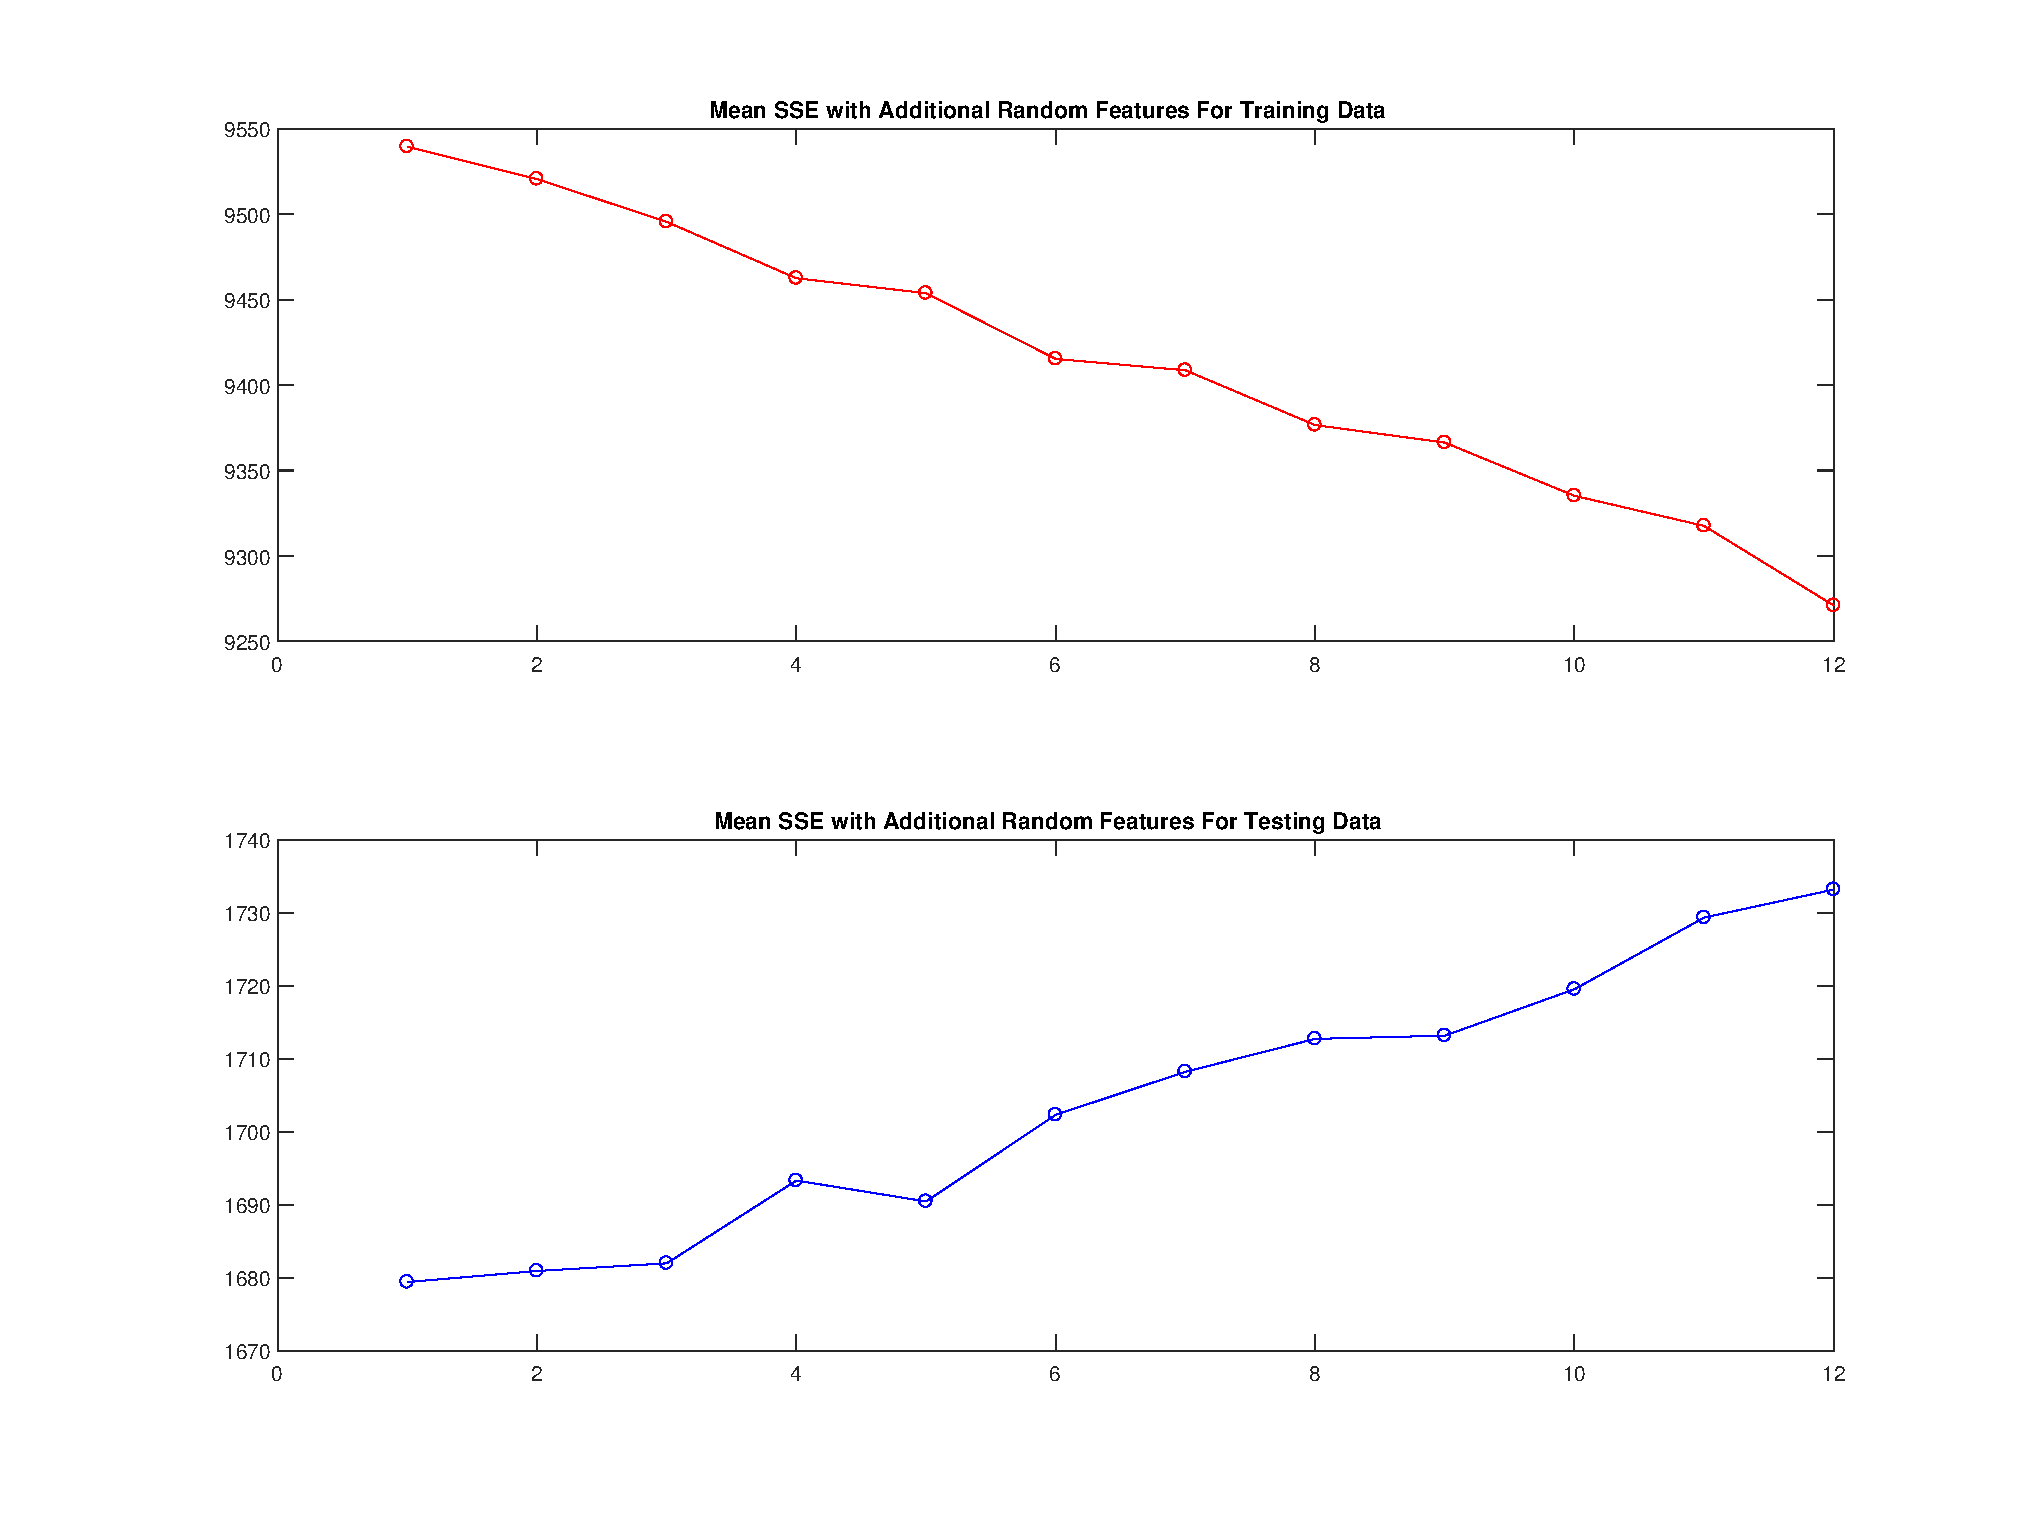
\includegraphics[scale=0.45]{random_figure.eps} 
		\end{center} 
		\label{fig:M1}
	\end{figure}
	
For the training data as we add more random features the SSE gets smaller. This makes sense since even though the features are randomly generated having more features allows our model to fit the training data closer. If we added random features until we had as many features as data points we would get a SSE of 0 for the training data. This of course would lead to incredible over fitting and we can see that trend in the testing SSEs. As we start adding more and more random features our testing SSE trends upwards.
	
	\newpage
	
	\section{Regularization}
	
We then returned to the original data set and calculated new Ws using the following formula:
	
	$$
	W = (X^{T}X + \lambda I)^{-1}X^{T}Y
	$$
	
For the vales of $\lambda$ s.t.:

$$
\lambda \in \{ 0.01, 0.05, 0.1, i^{i}, 0.5, 1, e, \pi, 5 \}
$$
	
We then calculated the SSEs for the testing and training data sets and plotted them:
	
	\begin{figure}[h!]
		\begin{center} 
			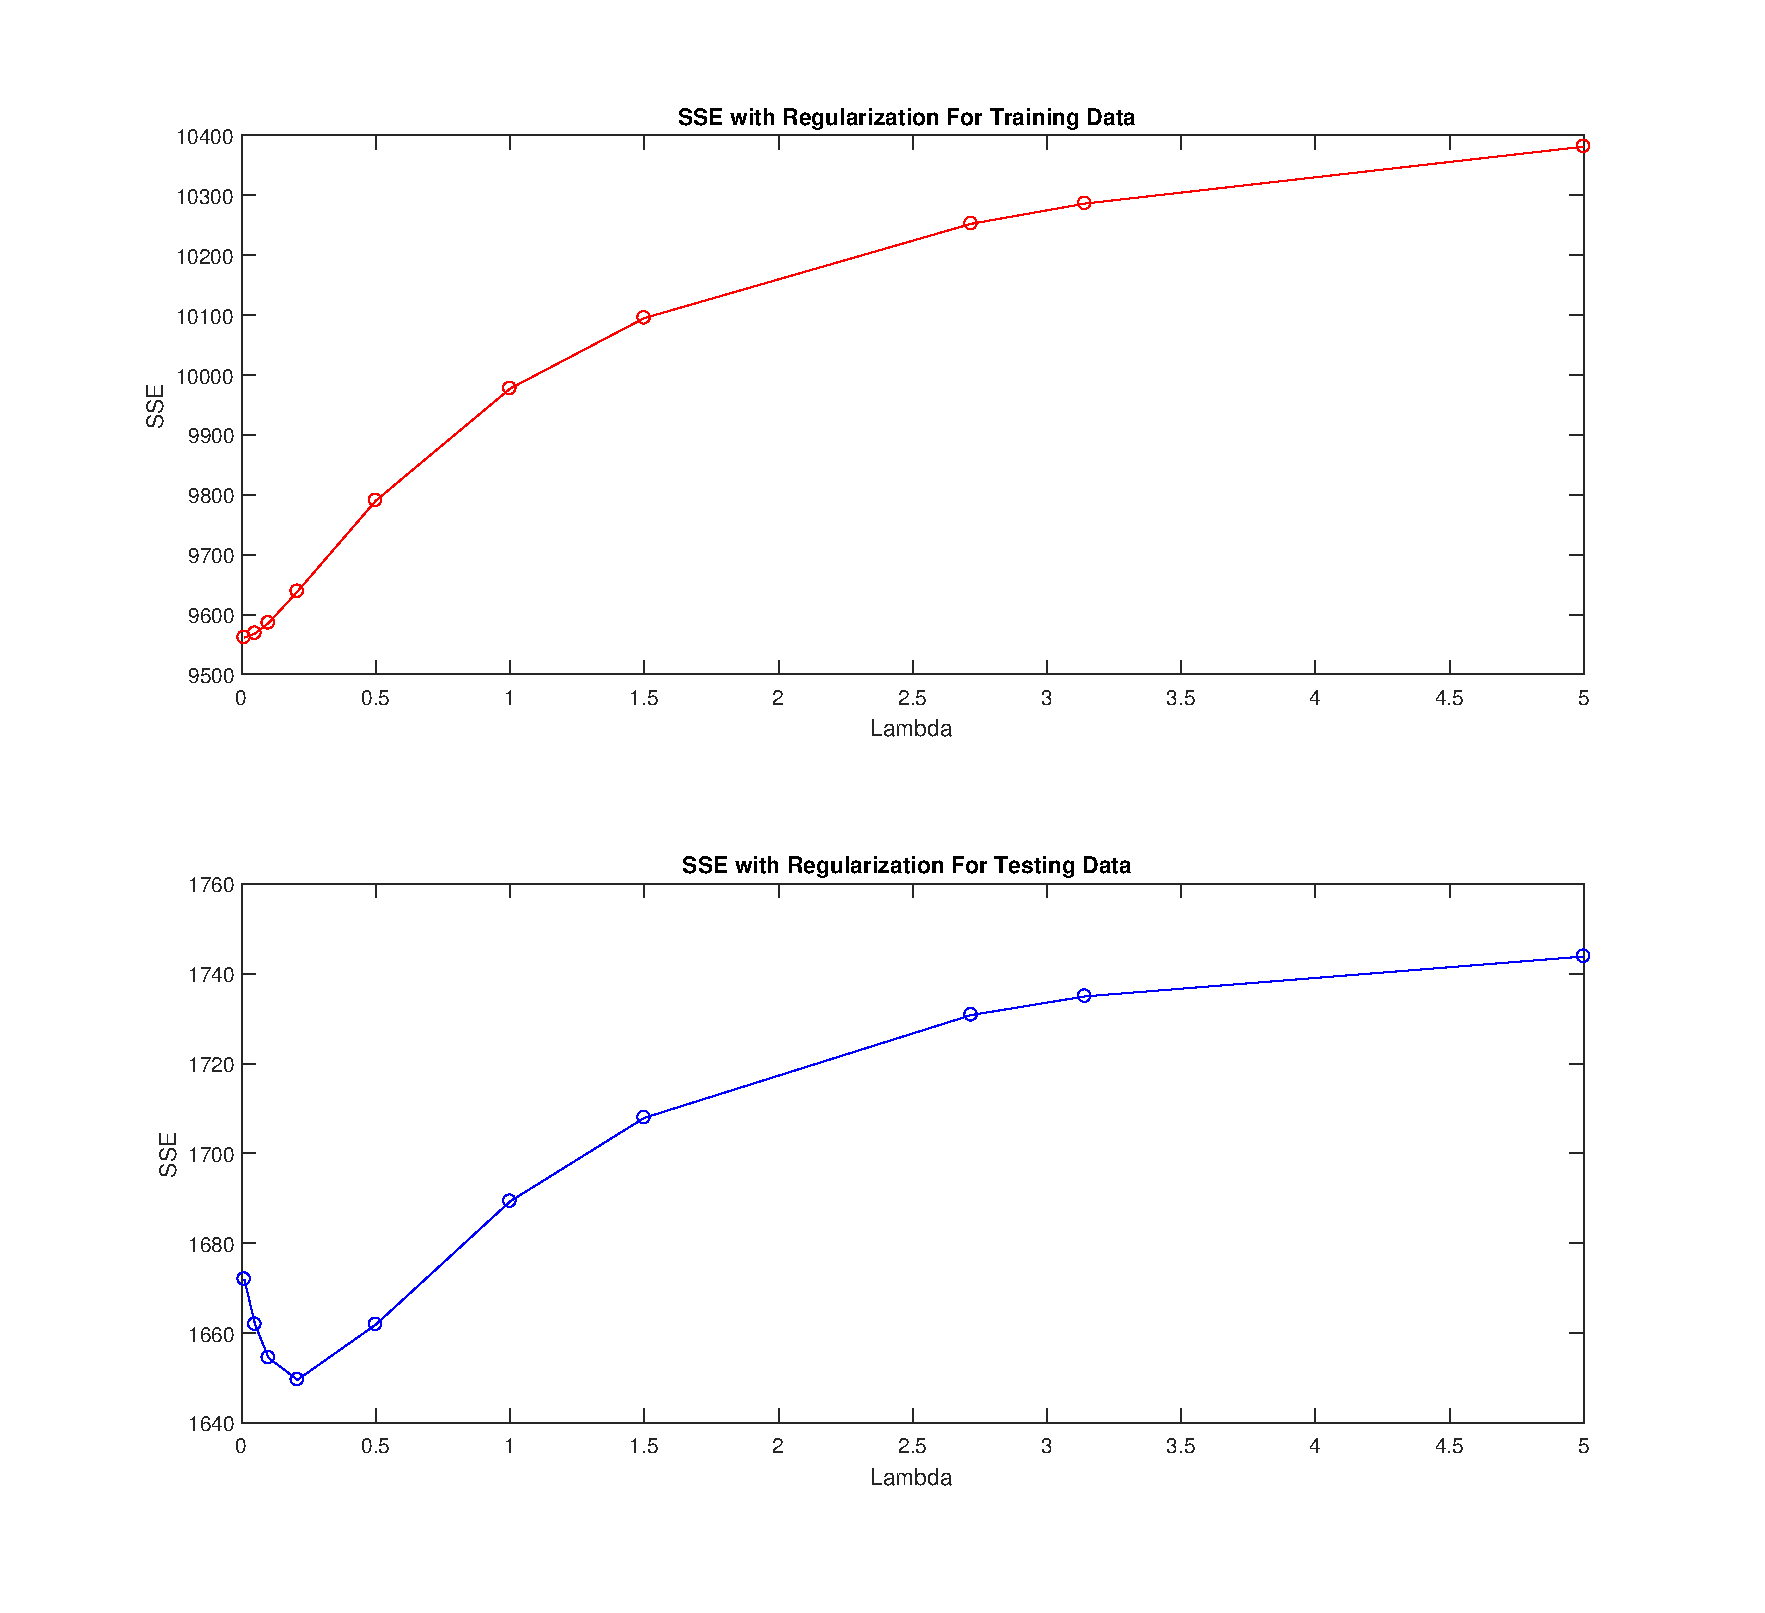
\includegraphics[scale=0.45]{lambda_figure.eps} 
		\end{center}  
		\label{fig:M2}
	\end{figure}

As we can see the SSEs for the training data gets larger as $\lambda$ get larger. This makes sense because as lambda increases the model under-fits our training data more and more. As we can see from the testing SSEs this starts out decreasing as lambda increases but after it peaks around $\lambda = i^{i}$ the SSEs start to increase. Thuus, from the values of $\lambda$ that we tried $i^i$ minimizes the testing SSE. \\ 
	
Also, as $\lambda$ increases we can see that the magnitude of the weights in W seem to be getting smaller overall. We can see this trend by plotting $\lambda$ and $\Vert W \Vert$:

	
	\begin{figure}[h!]
		\begin{center} 
			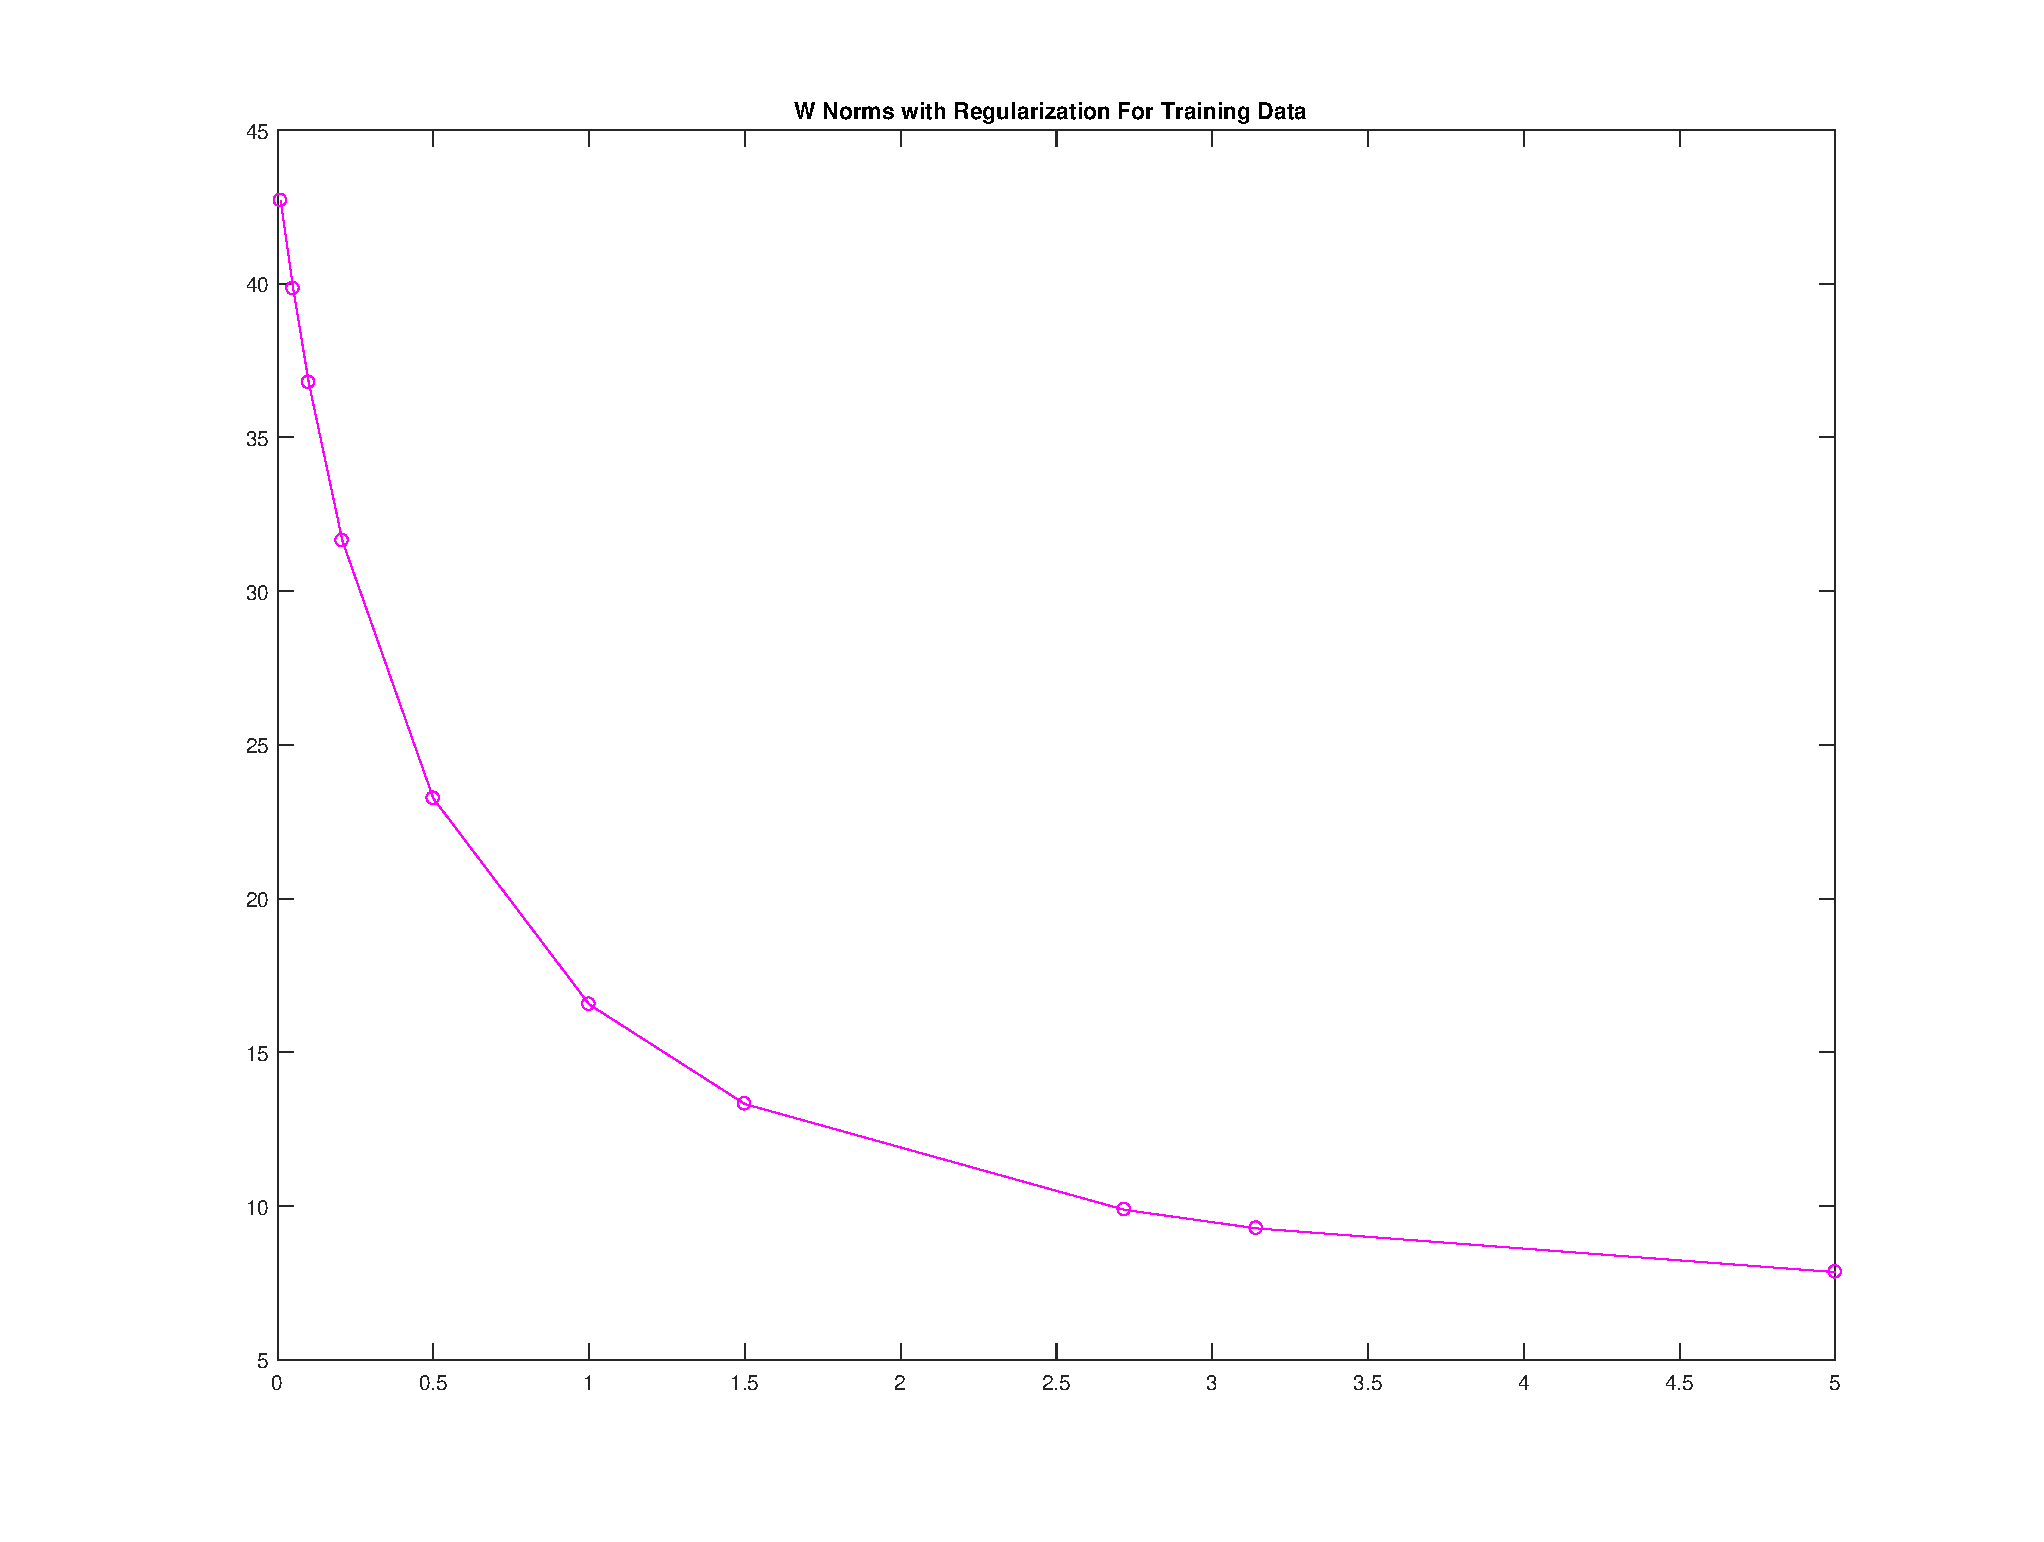
\includegraphics[scale=0.45]{lambda_norm.eps} 
		\end{center}  
		\label{fig:M3}
	\end{figure}
\newpage

We see a downward trend of $\Vert W \Vert$ as lambda decreases. This behavior makes sense when we consider that minimizing the equation: 

$$
\sum_{i = 1}^{n} (y_{i}-W^{T} x_{i})^{2} + \lambda \Vert W \Vert_{2}^{2}
$$

in terms of W is equivalent to solving the equation from above:

$$
W = (X^{T}X + \lambda I)^{-1}X^{T}Y
$$

As we can see in the former equation as $\lambda$ increases the minimization process is weighted more towards minimizing $\Vert W \Vert_{2}^{2}$ than $\sum_{i = 1}^{n} (y_{i}-W^{T} x_{i})^{2} = SSE$. Thus, as $\lambda$ increases $\Vert W \Vert_{2}^{2}$ will decrease which in turn decreases $\Vert W \Vert$. This is of course the pattern we saw in the above graph.
	
	
	\bibliography{myCitations} 
	\bibliographystyle{abbrv}
	
\end{document} 